\chapter{Intrabundle - An OSGi Bundle Introspection Tool}

\section{Introduction}

\section{Design Decisions}
To analyze large code bases of OSGi projects which can vary from KLOCs to thousands of KLOCs we needed a lightweight approach with the following functional requirements:

- 

The following alternatives were evaluated:

-

\section{JBoss Forge}

\section{Implementation Overview}

\section{Collecting Bundle Data}

\section{Metrics Calculation}

\section{Intrabundle Quality}
In this section we will see how intrabundle quality is managed and how some concepts of \textit{chapter 2 - State of art} were applied to the project.
\subsection{Internal quality}
Intrabundle internal is managed by PMD and JaCoCo. PMD is an static analysis tool and JaCoCo a dynamic analysis one. Both were presented at Chapter two in section \textit{Quality Analysis Tools} with the objective to guarantee non functional requirements.

\subsubsection{Example}
 A PMD was already illustrated at Chapter 2 as an example of static analysis tool. JaCoCo is used to calculate code coverage to track files and methods that automated tests are covering. Figure 3.1 shows JaCoCo code coverage report for Intrabundle:

\begin{figure}[h]
\caption{Intrabundle code coverage}
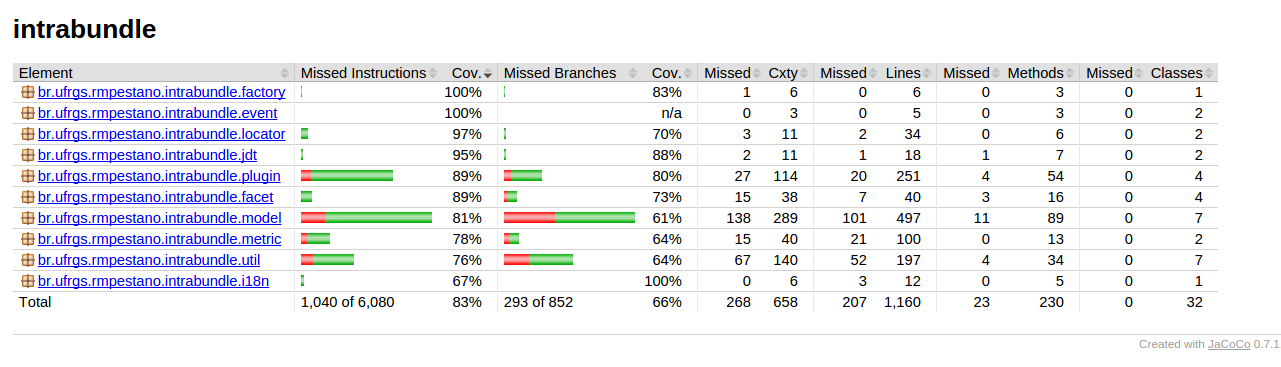
\includegraphics[scale=0.5]{intrabundle-code-coverage}
\end{figure}

\FloatBarrier

\subsection{External quality}
Intrabunde external quality is assured by automated whitebox tests so we can verify if Intrabundle is working as expected, if it meets its functional requirements.

\subsubsection{Example}
Intrabundle performs 62 \textbf{integration tests}, which can be defined as automated tests aimed to detect any inconsistencies between the software units that are integrated together, to guarantee its external quality. In this kind of automated tests the system must be running and in case of Intrabundle we also need the Forge runtime up and running during tests and that is done by Arquillian \citep{dan2011}, an integration test platform. Figure 3.2 shows the result of integration tests execution:

\begin{figure}[h]
\caption{Intrabundle external tests}
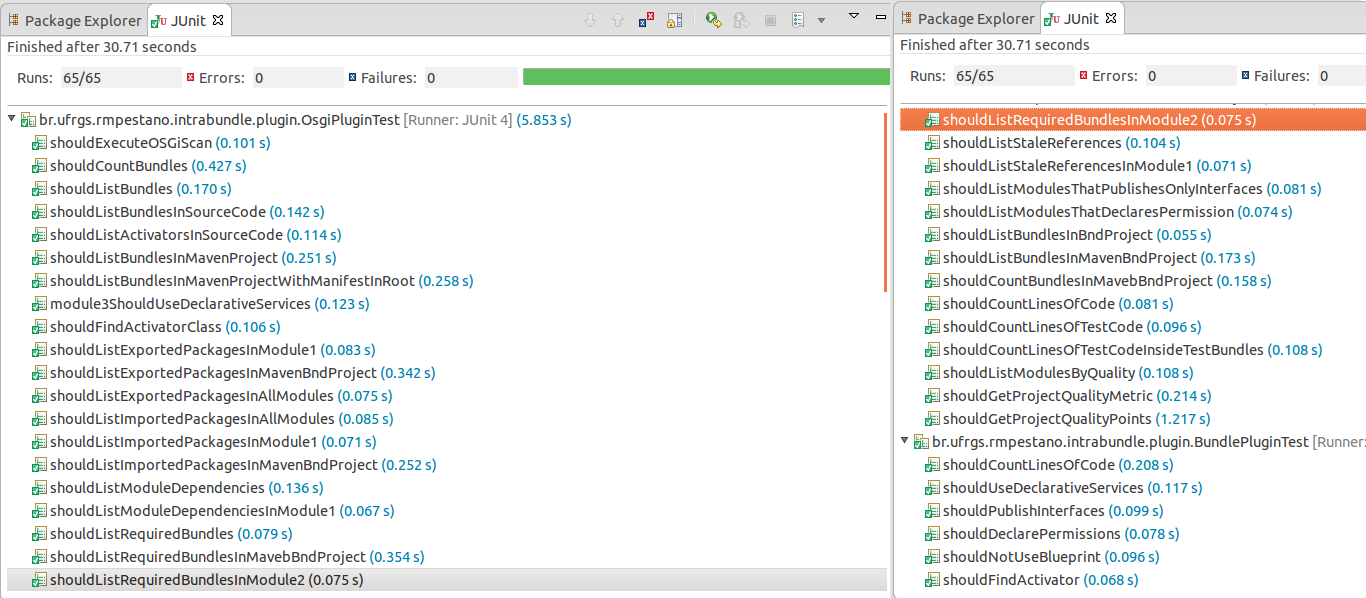
\includegraphics[scale=0.5]{intrabundle-external-quality}
\end{figure}

\FloatBarrier